\chapter{Recurrent Neural Networks}

\section{Introduction to Time Series}
A time series is a set of observations $\{x_t\}_{t \in \tau}$ collected over time. Based in the nature of $\tau$ we can distinguish between:
\begin{compactitemize}
    \item \textbf{Continuous time series}, when observation are made continuosly.
    \item \textbf{Discrete time series}, when the set of observation is finite. If the time delta between data points is fixed, the series is said to be regularly sampled with sampling frequecy $f_c = \frac{1}{\Delta t}$.
\end{compactitemize}
\begin{figure}[H]
    \centering
    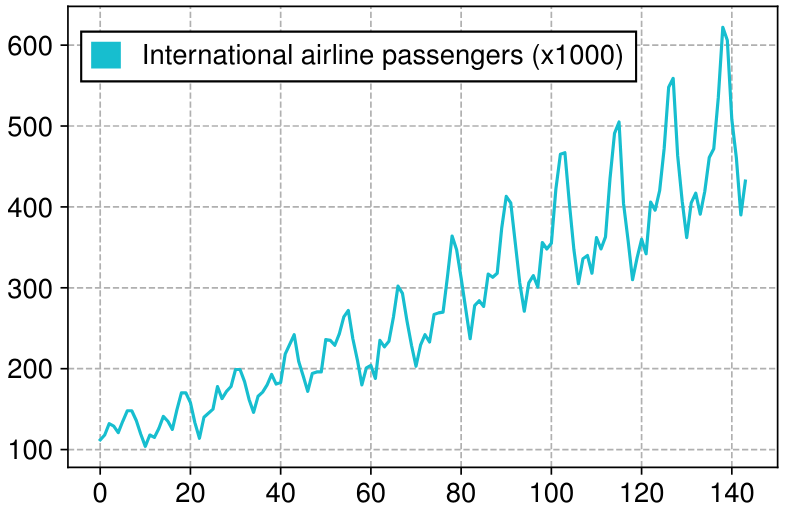
\includegraphics[width=0.6\textwidth]{images/series.png}
    \caption{Example of discrete and regulary sampled time series.}
    \label{fig:series}
\end{figure}
\begin{infobox}[Most important features of a time series]
    One important thing to note about the image above is that the series is composed of two characteristics: it increases over time and it oscillates. 
    If we focus on these aspects, we can notice that its behavior is periodic, and we can identify some important features:
    \begin{compactitemize}
        \item \textbf{Trend}: tendency of the series to increase or decrease over time.
        \item \textbf{Seasonality}: regular fluctuations that is more or less stable for each period of reference (e.g., daily, monthly, yearly).
        \item \textbf{Cyclic patterns}: periodic fluctuations around the trend.
        \item \textbf{Outliers}: values that appear out-of-distribution with respect to the rest of data.
        \item \textbf{Stationarity}: a stationary time series has statistical properties (mean, variance) that do not change over time. An example of a stationary series is a cosine or sine function.
    \end{compactitemize}
\end{infobox}

\subsection{STL Decomposition}
The \textbf{STL} decomosition split data into \textbf{S}easonality and \textbf{T}rend components using the \textbf{L}oess regression. The presence of a trend rules out the possibility that the series is stationary.
\begin{figure}[H]
    \centering
    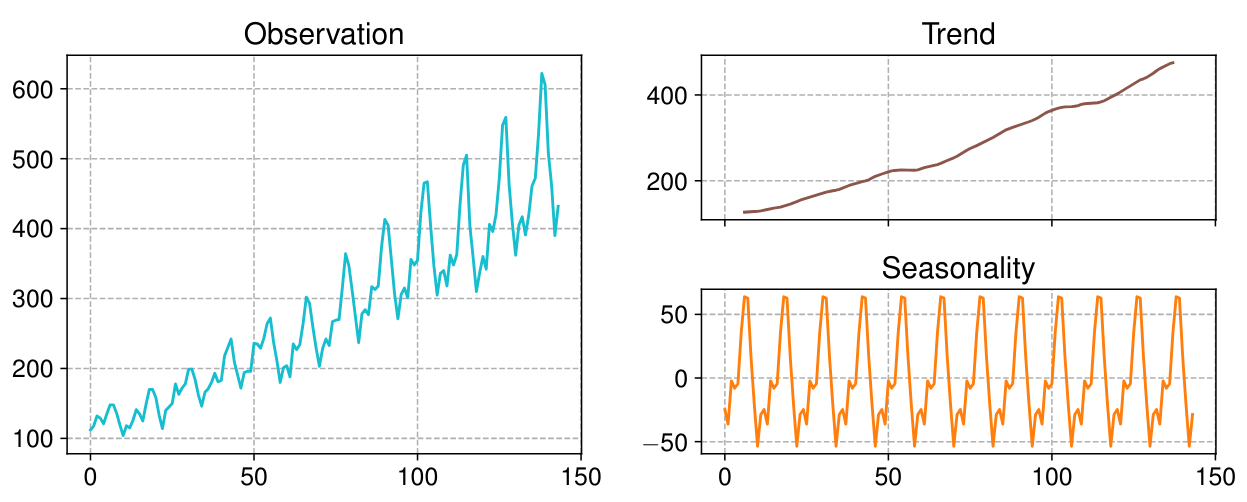
\includegraphics[width=0.9\textwidth]{images/STL_decomposition.png}
    \caption{Example of STL decomosition.}
    \label{fig:STL_decomosition}
\end{figure}

\begin{infobox}[Considerations]
    In this example, trend and seasonality components capture most of the patterns in the series. Noise and irregularities that cannot be decomposed are called \textbf{residuals} or \textbf{noise}. The residual is the difference between the original series and the sum of trend and seasonality (see Figure \ref{fig:Residuals}).
\end{infobox}
\begin{figure}[H]
    \centering
    \begin{minipage}{0.45\textwidth}
        \centering
        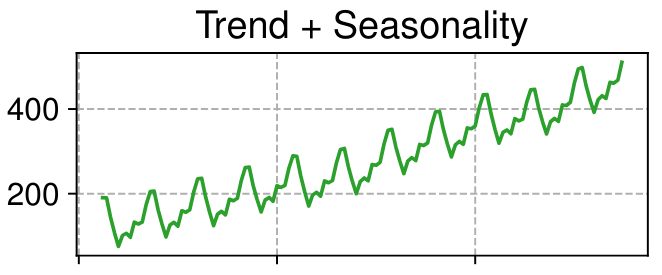
\includegraphics[width=\textwidth]{images/TS.png}
        \caption{Trend + Seasonality}
        \label{fig:Trend_Seasonality}
    \end{minipage}
    \hfill
    \begin{minipage}{0.45\textwidth}
        \centering
        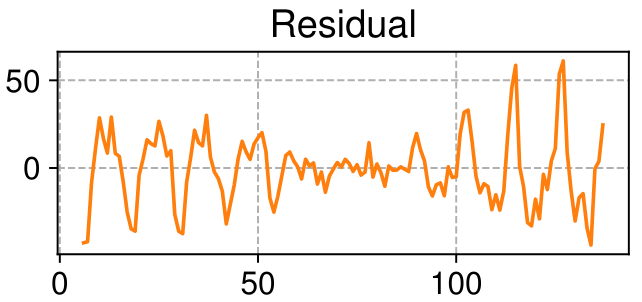
\includegraphics[width=\textwidth]{images/residual.png}
        \caption{Residuals}
        \label{fig:Residuals}
    \end{minipage}
    \label{fig:TS_Residuals}
\end{figure}

\section{Forecasting}
Having observed a time series over a period $\tau$ we want to estimate a future value (\textbf{forecast}) $\hat{x}_{\tau + h}$ with $h>0$. The value $h$ is called \textbf{forecast horizon}. To do that we can use:
\begin{compactitemize}
    \item \textbf{Data Generating Process (DPG):} essentialy we knew the process that had generated the data, and so it easy to make prediction. Obviously this is not the case in real life.
    \item \textbf{Approximate DGP:} we can try to approximate the DGP with a model, and use it to make prediction. This is the most common approach.
\end{compactitemize}
\begin{figure}[H]
    \centering
    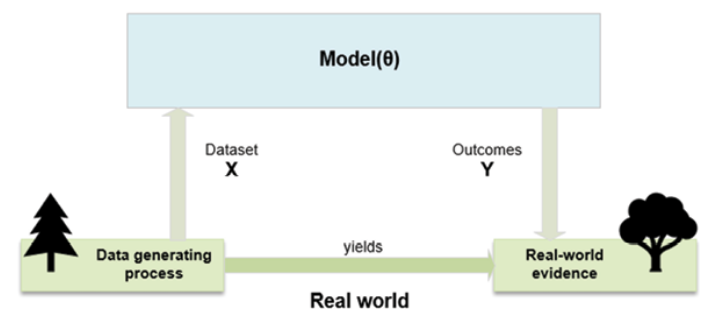
\includegraphics[width=0.7\textwidth]{images/forecasting.png}
    \caption{Idea of forecating should be.}
    \label{fig:forecasting}
\end{figure}

\begin{wrapfigure}{r}{0.35\textwidth}
    \centering
    \vspace{-10pt}
    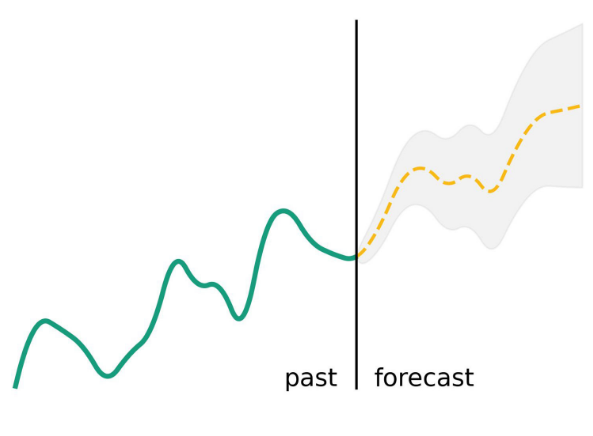
\includegraphics[width=\linewidth]{images/forecast_prediction.png}
    \caption{Example of forecast prediction.}
    \label{fig:forecast_prediction}
    \vspace{-10pt}
\end{wrapfigure}
Forecasting is used in many fields, such as:
\begin{compactitemize}
    \item \textbf{Finance:} Predict stock prices, bond yields, or currency exchange rates to guide investment strategies.
    \item \textbf{Retail:} Forecast demand to keep inventory levels optimal (avoid overstocking or stockouts).
    \item \textbf{Energy:} Predict eletricity load to balance grid supply and demand in real-time.
    \item \textbf{Words:} Predict the next word in a sentence for applications like text autocompletion and chatbots.
\end{compactitemize}

\subsection{Forecasting Problem}
Most forecasting models consider a limited window of past observations 
$\{x_t, x_{t-1}, \ldots, x_{t-q}\}$ and can be expressed as:
\[
x_t = f(x_{t-1}, \ldots, x_{t-q}; \boldsymbol{\phi}) 
    + g(\xi_{t-1}, \ldots, \xi_{t-q}; \boldsymbol{\theta})
\]

where $\xi_t, \ldots, \xi_{t-q}$ are random disturbances with mean $0$ and finite variance. 
The vectors $\boldsymbol{\phi}$ and $\boldsymbol{\theta}$ are the model parameters to be estimated.

The function $f(\cdot)$ captures the deterministic part of the model, describing how past observations influence the current value $x_t$. 
Conversely, the function $g(\cdot)$ introduces the stochastic component: 
since it depends on random noise terms $\xi_t$, it accounts for unpredictable fluctuations and uncertainty in the forecast. 
As a result, the prediction $\hat{x}_{\tau + h}$ is not purely deterministic, but inherently stochastic due to the influence of these random disturbances.
\begin{figure}[H]
    \centering
    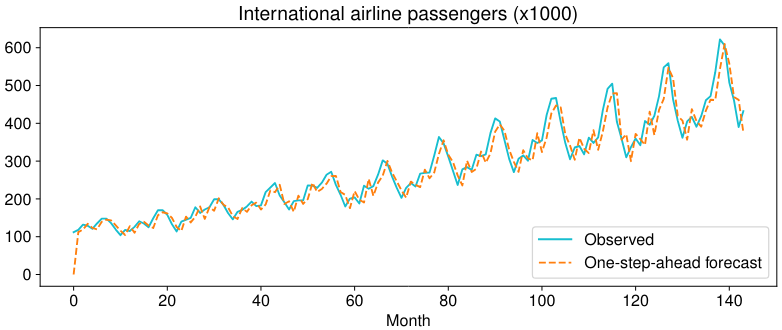
\includegraphics[width=0.85\textwidth]{images/F_problem.png}
    \caption{Another forecasting example.}
    \label{fig:forecasting}
\end{figure}

\subsection{Autoregressive Models}
An \textbf{autoregressive model} of order $p$, denoted as $\text{AR}(p)$, is defined as:
\[
x_t = \sum_{i=1}^{p} \phi_i x_{t-i} + \xi_t
\]
In this model, the current value $x_t$ is expressed as a linear combination of its $p$ most recent past values, plus a random disturbance term $\xi_t$.
\begin{compactitemize}
    \item The \textbf{order $p$} determines how many past observations are taken into account for the prediction. For example, an $\text{AR}(3)$ model depends on $x_{t-1}$, $x_{t-2}$, and $x_{t-3}$.
    \item The coefficients $\phi_i$ are the \textbf{learnable parameters} of the model, estimated from data to best capture the temporal dependencies.
    \item The term $\xi_t$ represents the \textbf{white noise}, i.e., random variations that are not explained by past values. It is typically modeled as a normal distribution:
    \[
    \xi_t \sim \mathcal{N}(0, \sigma^2)
    \]
    with mean $0$ and finite variance $\sigma^2$.
\end{compactitemize}
Thus, the autoregressive model captures the deterministic dependency of $x_t$ on its recent history through the parameters $\boldsymbol{\phi}$, while $\xi_t$ introduces the stochastic (random) component of the process.

\subsection{Moving Average Models}
A \textbf{moving average model} of order $q$, denoted as $\text{MA}(q)$, is defined as:
\[
x_t = \mu + \xi_t + \sum_{i=1}^{q} \theta_i \, \xi_{t-i}
\]
In this model, the current value $x_t$ is expressed as a linear combination of the last $q$ random shocks (or errors), plus the mean of the series.
\begin{compactitemize}
    \item The \textbf{order $q$} determines how many past random variations (errors) are taken into account. For example, an $\text{MA}(2)$ model depends on $\xi_{t-1}$ and $\xi_{t-2}$.
    \item The parameter $\mu$ represents the \textbf{mean level} of the time series, often estimated as the empirical mean of $\{x_t\}_{t \in \tau}$.
    \item The coefficients $\theta_i$ are the \textbf{learnable parameters} of the model, which determine how much influence each past error has on the current value.
    \item The terms $\xi_{t-i}$ represent the \textbf{previous random shocks} or error terms, typically modeled as white noise:
    \[
    \xi_t \sim \mathcal{N}(0, \sigma^2)
    \]
    with mean $0$ and finite variance $\sigma^2$.
\end{compactitemize}
Thus, the moving average model captures the stochastic dependency of $x_t$ on past random variations, rather than on past observed values. The process is therefore driven by recent shocks, weighted by the parameters $\boldsymbol{\theta}$.

\subsection{ARMA Models}
An \textbf{autoregressive moving average model} of order $(p,q)$, denoted as $\text{ARMA}(p,q)$, combines the features of both AR and MA models:
\[
x_t = \sum_{i=1}^{p} \phi_i x_{t-i} + \xi_t + \sum_{j=1}^{q} \theta_j \, \xi_{t-j}
\]
\begin{compactitemize}
    \item The \textbf{AR part of order $p$} captures the linear dependence of $x_t$ on its $p$ most recent past values.
    \item The \textbf{MA part of order $q$} captures the influence of the last $q$ random shocks on $x_t$.
    \item The parameters $\phi_i$ and $\theta_j$ are \textbf{learnable} and estimated from the data.
    \item The noise term $\xi_t$ is modeled as \textbf{white noise} with mean $0$ and variance $\sigma^2$.
\end{compactitemize}
The ARMA model is suitable for \textbf{stationary time series} where both past values and past shocks contribute to the dynamics of the process.

\begin{infobox}[Note about the need of stationarity]
    Autoregressive (AR), Moving Average (MA) and Autoregressive Moving Average (ARMA) models require the underlying time series to be \textbf{stationary}. This is because:
    \begin{compactitemize}
        \item \textbf{AR models} assume that the linear dependence on past values is stable over time. If the mean or variance of the series changes, the learned coefficients would not correctly capture the relationships.
        \item \textbf{MA models} assume that past shocks (errors) have constant variance and zero mean. Non-stationarity would make the influence of past errors unpredictable.
        \item \textbf{ARMA models} combine AR and MA parts, so they inherit the same requirements: the series must have a \textbf{constant mean, constant variance, and autocorrelations that depend only on lag} (weak stationarity).
    \end{compactitemize}
    \textbf{Key point:} Most real-world series are not stationary (they may have trends, seasonality, or changing variance). Before fitting AR, MA, or ARMA models, the series is often transformed to stationarity via \textbf{differencing}, \textbf{detrending}, or variance-stabilizing transformations. Only after this step do these models provide reliable approximations and forecasts.
\end{infobox}
    
\section{Data Pre-processing}
\begin{wrapfigure}{r}{0.4\textwidth}
    \centering
    \vspace{-10pt}
    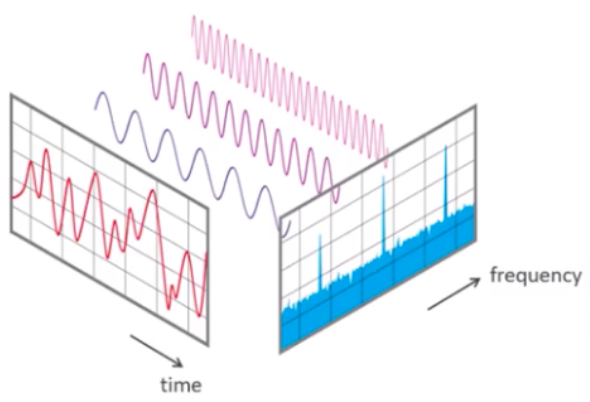
\includegraphics[width=\linewidth]{images/FT.png}
    \caption{Fourier Transform.}
    \label{fig:forecast_prediction}
    \vspace{-10pt}
\end{wrapfigure}
Preprocessing is a crucial step when working with time series data. Unlike regular datasets, time series have a temporal structure that must be preserved and carefully handled. This means that before feeding data into any model, we need to ensure that time information is properly extracted, formatted, and refined.  
High-level preprocessing techniques can be applied depending on the nature of the series:  
\begin{compactitemize}
    \item \textbf{Linear methods} like Fourier Transform or Wavelet Transform, which help in analyzing periodicities and trends.  
    \item \textbf{Non-linear methods:} Hilbert-Huang Transform (HHT).  
\end{compactitemize}

\begin{infobox}[Use Fourier Transformation to Detect Engine Vibrations]
    The \textbf{Fourier Transform} is a powerful tool for analyzing the frequency content of a signal. In practical applications, such as monitoring engine vibrations, it helps identify periodic components that may indicate mechanical issues.  
    
    \begin{compactitemize}
        \item Each mechanical part of an engine tends to vibrate at characteristic frequencies under normal operation.  
        \item By applying the Fourier Transform to vibration data, we can convert the time-domain signal into the frequency domain and identify dominant frequency components.  
        \item \textbf{Abnormal vibrations} often appear as unexpected peaks at frequencies that do not correspond to normal engine operation. For example, a broken bearing or imbalance in a rotor can generate vibrations at specific frequencies.  
        \item Detecting these unusual frequency peaks allows engineers to diagnose potential faults early, before they cause severe damage.  
    \end{compactitemize}
    
    \textbf{Key point:} Fourier analysis is most useful when the problem involves periodic or quasi-periodic signals. In the context of engines, it helps pinpoint which components might be failing based on the frequency patterns of the vibrations.
\end{infobox}
    

\subsection{Data Preparation}
Time series data cannot just be treated like a normal dataset. In the sense, to make predictions we need to have numbers that represent the information, for example the following table
\begin{table}[h!]
    \centering
    \begin{tabular}{|c|c|}
    \hline
    \textbf{Month} & \textbf{Passengers} \\
    \hline
    1949-01 & 112.0 \\
    1949-02 & 118.0 \\
    1949-03 & 132.0 \\
    1949-04 & 129.0 \\
    1949-05 & 121.0 \\
    \hline
    \end{tabular}
\end{table}
represent a time series of monthly airline passengers. if we want make prediction we must transfor data such dates into numerical values. 
\newpage
\subsection{Cyclical Features}
\begin{wrapfigure}{r}{0.2\textwidth}
    \centering
    \vspace{-10pt}
    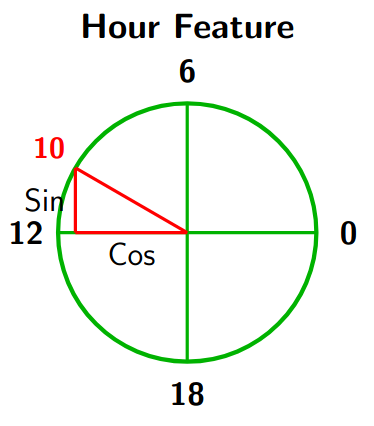
\includegraphics[width=\linewidth]{images/circle.png}
    \label{fig:cyclical_features}
    \vspace{-10pt}
\end{wrapfigure}
Some time-related features are \textbf{cyclical} (e.g., hours of the day, months of the year) and should preserve their periodicity for models to capture patterns correctly:
\begin{compactitemize}
    \item Neural networks work better when inputs have \textbf{zero mean} and \textbf{fixed variance}.  
    \item Cyclical features can be encoded on the \textbf{unit circle} using sine and cosine transformations:
    \[
    \text{Sin(hour)} = \sin\left(\text{hour} \cdot \frac{2\pi}{24}\right), \quad
    \text{Cos(hour)} = \cos\left(\text{hour} \cdot \frac{2\pi}{24}\right)
    \]
    \item The same approach can be applied to months (1--12) or other cyclical variables.
\end{compactitemize}

\section{Recurrent Neural Networks (RNNs)}
Feedforward neural networks (MLPs) compute outputs by propagating information directly from the input $x$ through intermediate hidden layers $h$ to the output $y$. These networks require a fixed-size input because each input neuron corresponds to a specific component of the input vector. In contrast, some network topologies include feedback connections, where outputs are fed back into the network itself. This defines the family of \textbf{Recurrent Neural Networks (RNNs)}, which are specialized for processing sequences. Unlike feedforward networks, RNNs can handle variable-length sequences in the input, in the output, or both, thanks to their internal state that summarizes the sequence seen so far. It is important to note that RNNs are not an architecture per se, but rather a framework that can be implemented in various ways.
\begin{figure}[H]
    \centering
    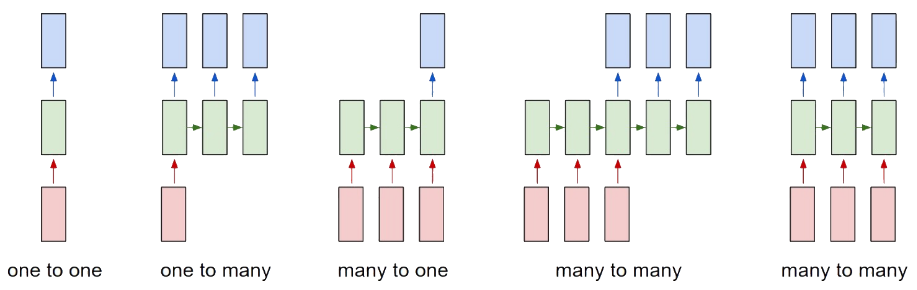
\includegraphics[width=0.85\textwidth]{images/RNN_framwork.png}
    \caption{RNN framework.}
    \label{fig:RNN_framework}
\end{figure}
\begin{infobox}[What is meant by "different size input"]
    Typically, in a \textbf{feedforward neural network (MLP)}, the input must have a \textbf{fixed size}, meaning that the number of input neurons is predetermined and cannot change. Each input neuron corresponds to a specific feature, so if the input vector changes in length, the network cannot process it correctly. Moreover, \textbf{MLPs process the entire input at once} in a single forward pass, without any notion of sequential order.
    
    For example, to predict the next word given a sequence of 5 words, an MLP would require all 5 word embeddings concatenated into a single large input vector. This means the input size grows linearly with the sequence length, making it impractical for long sequences.
    
    In contrast, \textbf{Recurrent Neural Networks (RNNs)} can handle \textbf{sequences of variable length} because they process the input one element at a time and maintain a hidden state that summarizes the information seen so far. In the same prediction task, an RNN would process each word sequentially, updating its hidden state at each step. While each individual element in the sequence must have a fixed dimensionality, the \textbf{number of elements} (i.e., the sequence length) can vary. This allows RNNs to effectively manage sequences of different lengths, as the hidden state carries forward information from earlier timesteps.
\end{infobox}

\subsection{Vanilla RNN}
\begin{wrapfigure}{r}{0.15\textwidth}
    \centering
    \vspace{-10pt}
    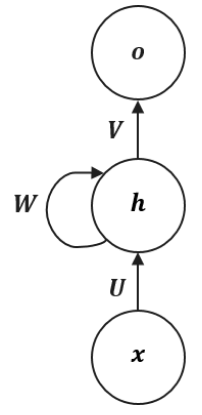
\includegraphics[width=\linewidth]{images/vanilla_RNN.png}
    \label{fig:forecast_prediction}
    \vspace{-10pt}
\end{wrapfigure}
The vanilla RNN is provided with three sets of parameters:
\begin{compactitemize}
    \item $\mathbf{U}$: weights connecting the input $\mathbf{x}_t$ to the hidden state $\mathbf{h}_t$.
    \item $\mathbf{W}$: weights connecting the previous hidden state $\mathbf{h}_{t-1}$ to the current hidden state $\mathbf{h}_t$.
    \item $\mathbf{V}$: weights connecting the hidden state $\mathbf{h}_t$ to the output $\mathbf{o}_t$.
\end{compactitemize}
System dynamics are defined by the following equations:
\[
h^{(t)} = \phi\big(W \, h^{(t-1)} + U \, x^{(t)}\big)
\]
\[
o^{(t)} = V \, h^{(t)}
\]

where $\phi(\cdot)$ is a non-linear activation function, typically $\tanh$ or ReLU. The hidden state $h^{(t)}$ acts as the network's memory, capturing information from previous timesteps. The output $o^{(t)}$ is computed from the current hidden state.

The hidden state $h^{(t)}$ can be intuitively viewed as a \textbf{lossy summary} of the sequence of past inputs fed to the network, in which the main task-relevant aspects of the past sequence of inputs up to time $t$ are stored.  

Since an input sequence of arbitrary length $(x^{(1)}, x^{(2)}, \dots, x^{(t)})$ is mapped into a fixed-size vector $h^{(t)}$, this summary is necessarily \textbf{lossy}.
\begin{infobox}[Important note]
    The parameters $\mathbf{U}$, $\mathbf{W}$, and $\mathbf{V}$ are \textbf{shared across all timesteps}. This weight sharing is crucial because it allows the RNN to generalize across different positions in the sequence. The same transformation is applied at each timestep, enabling the network to learn temporal patterns that are independent of the absolute position in the sequence.
\end{infobox}

\subsection{Training RNNs}
A recurrent computational graph can be unfolded into a sequential computational graph with a respective structure. The output at each timestep is obtained like that:
\[
h^{(t)} = f(h^{(t-1)}, x^{(t)}; \theta)
\]
\begin{figure}[H]
    \centering
    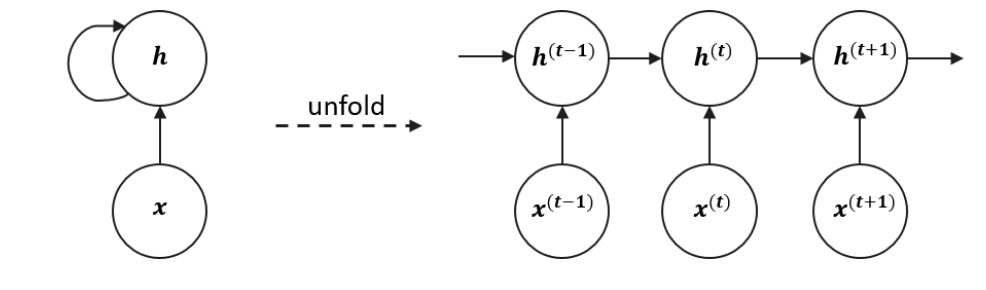
\includegraphics[width=0.65\textwidth]{images/RNN_unfolded.png}
    \caption{RNN unfolded.}
    \label{fig:RNN_unfolded}
\end{figure}
The capacity to unfold a recurrent graph into a DAG (Directed Acyclic Graph) allows for
training a recurrent neural network using standard backpropagation.
Because the gradient conceptually flows backwards through time instead of through layers, this
algorithm is usually referred to as \textbf{backpropagation through time (BPTT)}.

Let's make an example for a simple architecture which processes sequences of length $\tau=3$ and produces an output at the end of the sequence.
\begin{figure}[H]
    \centering
    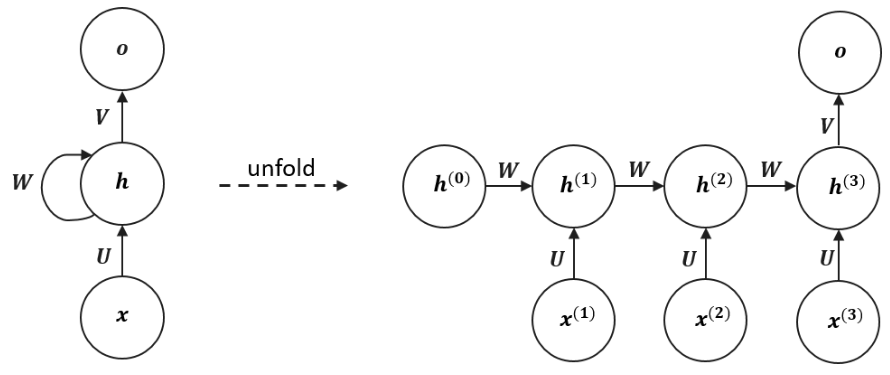
\includegraphics[width=0.65\textwidth]{images/RNN_unfolded_output.png}
    \caption{RNN unfolded with output.}
    \label{fig:RNN_unfolded}
\end{figure}

Now, given a differentiable loss on final output $L(y,o)$,let's compute the derivate of the objective $L$ with respect to the weights $ V, W and U$ and see what happends. The gradients that we must compute is:
\[
\frac{\partial L}{\partial V} = \frac{\partial L}{\partial o} \frac{\partial o}{\partial V}
\]
\[
\frac{\partial L}{\partial W} = \frac{\partial L}{\partial o} \frac{\partial o}{\partial h^{(3)}} 
\sum_{k=0}^{3} \left[ \frac{\partial h^{(3)}}{\partial h^{(k)}} \frac{\partial h^{(k)}}{\partial W} \right]
\]
\[
\frac{\partial L}{\partial U} = \frac{\partial L}{\partial o} \frac{\partial o}{\partial h^{(3)}} 
\sum_{k=0}^{3} \left[ \frac{\partial h^{(3)}}{\partial h^{(k)}} \frac{\partial h^{(k)}}{\partial U} \right]
\]
The first gradient depends only on current state, the other two depend on all previous states.

\textbf{Note:} The calculation of the gradient with respect to $W$ is performed only once, because $W$ is \textbf{shared across all timesteps}!!
\begin{infobox}[Compute the derivatives of $h^{(3)}$ with respect to $h^{(0)}$]
    Consider a simple RNN unrolled over 3 timesteps:
    \[
    h^{(t)} = \phi\big(W h^{(t-1)} + U x^{(t)}\big)
    \]
    with $\phi(\cdot)$ being the ReLU activation function.  
    
    Assume that ReLU is \textbf{always active} (i.e., never zero), so the derivative of $\phi$ is 1 for all units. Then, the derivative of the hidden state at timestep 3 with respect to the initial hidden state $h^{(0)}$ is:
    
    \[
    \frac{\partial h^{(3)}}{\partial h^{(0)}} 
    = \frac{\partial h^{(3)}}{\partial h^{(2)}} \frac{\partial h^{(2)}}{\partial h^{(1)}} \frac{\partial h^{(1)}}{\partial h^{(0)}} = W \cdot W \cdot W = W^3
    \]
    
    \textbf{Implications:}
    
    \begin{compactitemize}
        \item If the values in $W$ are less than 1, raising them to a power (as in $W^3$) makes them even smaller, causing the gradient to shrink as it propagates backward. This is the \textbf{vanishing gradient} problem.
        \item If the values in $W$ are greater than 1, raising them to a power makes them larger, causing the gradient to grow as it propagates backward. This is the \textbf{exploding gradient} problem.
        \item This explains why training vanilla RNNs over long sequences is difficult: the gradient can either vanish or explode, making it hard to learn long-term dependencies.
    \end{compactitemize}
    
    \textbf{Note:} so the part of the update that might be problematic is:
    \[
    \frac{\partial h^{(3)}}{\partial h^{(k)}}
    \]

    \textbf{Note for the exam:} The professor might ask you to compute the derivatives of some functions. So be sure to know how to do it.
\end{infobox}

\subsection{The Challenge of Long-Term Dependencies: Vanishing Gradients}
Looking closer at RNNs, we notice that the gradient at a given timestep depends on gradients at previous timesteps, computed recursively through the chain rule. When using activation functions like \texttt{tanh} or \texttt{sigmoid}, the effect of each timestep on the gradient is naturally limited: for \texttt{tanh} the maximum contribution is 1, and for \texttt{sigmoid} it is even smaller. As a result, when we multiply these contributions across many timesteps, the gradient can shrink rapidly, effectively becoming zero. This phenomenon is known as the \textbf{vanishing gradient problem} and it creates major difficulties in learning long-term dependencies, because the influence of “far-away” timesteps essentially disappears during training.
\subsection{The Challenge of Long-Term Dependencies: Exploding Gradients}
Depending on the network parameters and the choice of activation functions, the opposite problem can occur: the \textbf{exploding gradient problem}. In this case, gradients grow larger and larger as they are propagated backward, eventually causing numerical instability and preventing proper optimization. Both vanishing and exploding gradients can be mitigated through careful weight initialization, the selection of suitable activation functions, and techniques like gradient clipping. While these issues can also appear in deep feedforward networks, they are especially common in recurrent architectures, since an RNN unrolled over time is effectively as deep as the length of the input sequence.
\begin{infobox}[Where do we stop learning?]
    In the vanishing gradient problem, the weights that stop learning are those in the first layers,
    because the gradient becomes smaller and smaller as we go back in time.
    Thus, the weights that are updated the least are those furthest back in time:
    the model gradually forgets older information.

    In the exploding gradient problem, the gradients grow larger and larger as we go back in time.
    As a result, the early weights (those furthest back in time) receive excessively large updates,
    which can dominate the learning process and make the later weights almost irrelevant.
    The model becomes unstable and struggles to learn recent information properly.
\end{infobox}


\section{Advanced Recurrent Architectures}
\textbf{Long Short-Term Memory (LSTM)} and \textbf{Gated Recurrent Unit (GRU)} are more complex recurrent architectures that have been proposed to overcome the issues in the gradient flow and to ease the learning of long-term dependencies thanks to the introduction of \textbf{learnable gating mechanism}.
\begin{figure}[H]
    \centering
    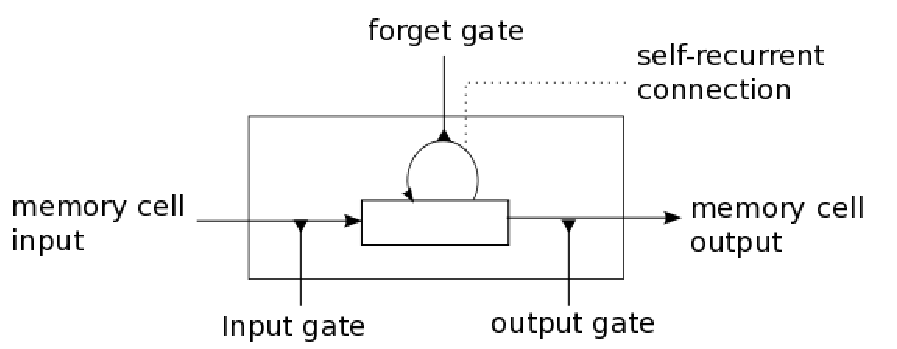
\includegraphics[width=0.6\textwidth]{images/gate.png}
    \caption{Illustration of a learnable gating mechanism used in LSTM and GRU architectures, which controls the flow of information and helps mitigate vanishing and exploding gradient problems.}
    \label{fig:gate}
\end{figure}

\subsection{Long Short-Term Memory networks}
The \textbf{Long Short-Term Memory (LSTM)} network introduces a set of learnable gates that control the flow of information, allowing the network to maintain long-term dependencies more effectively than a vanilla RNN. The main components are the \textbf{input gate} $i$, the \textbf{forget gate} $f$, the \textbf{output gate} $o$, the candidate cell state $\tilde{C}$, the cell state $C^{(t)}$, and the hidden state $h^{(t)}$.  
\begin{figure}[H]
    \centering
    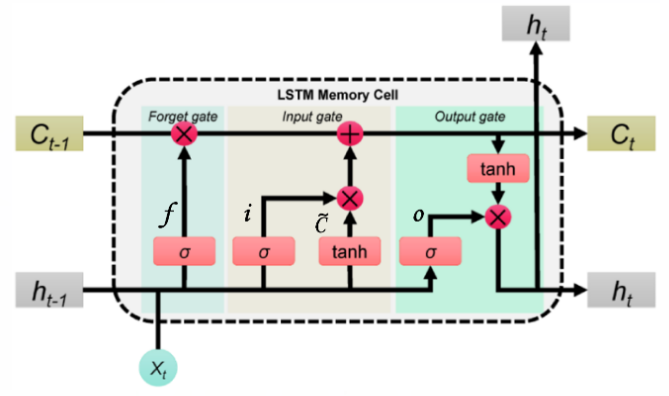
\includegraphics[width=0.65\textwidth]{images/LSTM_model.png}
    \caption{LSTM model.}
    \label{fig:RNN_unfolded}
\end{figure}

The update equations can be compactly written as:
\[
\left\{
\begin{aligned}
i &= \sigma\big(x^{(t)} U_i + h^{(t-1)} W_i\big) \\
f &= \sigma\big(x^{(t)} U_f + h^{(t-1)} W_f\big) \\
o &= \sigma\big(x^{(t)} U_o + h^{(t-1)} W_o\big) \\
\tilde{C} &= \tanh\big(x^{(t)} U_C + h^{(t-1)} W_C\big) \\
C^{(t)} &= C^{(t-1)} \odot f + \tilde{C} \odot i \\
h^{(t)} &= \tanh\big(C^{(t)}\big) \odot o
\end{aligned}
\right.
\]
where $\odot$ denotes element-wise multiplication and $\sigma$ is the sigmoid activation function.  

\textbf{Explanation:}
\begin{compactitemize}
    \item The \textbf{input gate} $i$ controls how much of the candidate cell state $\tilde{C}$ should be added to the cell state.
    \item The \textbf{forget gate} $f$ decides how much of the previous cell state $C^{(t-1)}$ should be retained.
    \item The \textbf{output gate} $o$ regulates how much of the cell state is exposed to the hidden state $h^{(t)}$.
    \item The \textbf{cell state} $C^{(t)}$ acts as the memory of the LSTM, accumulating information over time.
    \item The \textbf{hidden state} $h^{(t)}$ is the output at the current timestep, which also feeds into the next timestep.
\end{compactitemize}
These equations allow LSTMs to selectively remember or forget information at each timestep, addressing the vanishing and exploding gradient problems typical of vanilla RNNs.

\begin{infobox}[The calculus of \texorpdfstring{$\tilde{C}$, $C^{(t)}$ and $h^{(t)}$}{tilde C, C(t) and h(t)}]
    The candidate cell state is computed as:
    \[
    \tilde{C} = \tanh\big(x^{(t)} U_C + h^{(t-1)} W_C\big)
    \]
    The equation is pretty much the same as that we saw in for vanilla RNN architecture. Nonetheless, the amount of influence of $\tilde{C}$ on the LSTM memory cell is controlled by the input gate $i$.

    The update for the update memoruìy cell $C^{(t)}$ is:
    \[
    C^{(t)} = C^{(t-1)} \odot f + \tilde{C} \odot i
    \]
    The forget gate $f$ controls  how much of the memory from previous steps $C^{(t)}$ is retained, while the input gate $i$ supervises the amount of newly computed state $\tilde{C}$ that has to flow into the memory.

    Finally, the hidden state $h^{(t)}$ is computed as:
    \[
    h^{(t)} = \tanh\big(C^{(t)}\big) \odot o
    \]
    The output gate $o$ regulates how much of the cell state $C^{(t)}$ is exposed to the hidden state $h^{(t)}$. The $\tanh$ activation ensures that the values remain bounded between -1 and 1.

    \textbf{Note:} The gate $i$, $f$ and $o$ are \emph{vector} of the same size as the cell state $C$, this insure that multiplication is element-wise. 
\end{infobox}
\newpage
The cell has two inner states:
\begin{compactitemize}
    \item The cell state $C$ represent the \textbf{long-term memory} of the network, and can hold past information without being overwritten quickly.
    \item The hidden state $h$, which also acts as the output, represent the \textbf{short-term memory}; it changes frequently, reflecting the most recent processing, thus containing the information needed for the prediction of the current time step.
\end{compactitemize}


